\documentclass[12pt]{article}
\usepackage[utf8]{inputenc}
\usepackage[T1]{fontenc}
\usepackage{geometry}
\usepackage{graphicx}
\usepackage{makeidx}
\geometry{margin=2.5cm}

\title{Informe - Práctica \#1}
\author{Tu nombre}
\date{Fecha de entrega}

\begin{document}

	\thispagestyle{empty}
	
	\begin{center}
		
\includegraphics[width=3.1cm,height=2cm]{logo}\\
		UNIVERSIDAD SIMÓN BOLÍVAR\\
		DEPARTAMENTO DE ELECTRÓNICA Y CIRCUITOS\\
		EC1281 - LABORATORIO DE MEDICIONES ELÉCTRICAS\\
		SECCIÓN 1 - GRUPO 1\\
		
		\vspace{7cm}
		\textbf{\Large INFORME - PRÁCTICA \#1}\\
		INTRODUCCIÓN AL LABORATORIO\\
	\end{center}

	\begin{flushleft}
		\vspace{9cm}
		\hfill Integrantes:\\
		\hfill {\large Luis Becerra - 1910557}\\
		\hfill {\large Lorena Rojas - 1910469}\\
	\end{flushleft}

	\newpage
	
	\pagenumbering{roman}
	
	\begin{center}
		\textbf{\large RESUMEN}\\
	\end{center}
	
	En esta práctica de laboratorio se realizó una introducción al laboratorio de mediciones eléctricas, aprendiendo acerca del tablero de breckets y el mesón de trabajo, así como las normas de seguridad necesarias para trabajar con estos equipos. Además, se identificaron las herramientas que se encontraban en el mesón de trabajo, tales como el computador, el variac, el multimetro, potenciometros, osciloscopios, entre otros. A continuación, se procedió a realizar mediciones con el multimetro a las resistencias y potenciometros disponibles, con el objetivo de comprender cómo funcionan y cómo se comportan estos componentes eléctricos. Esta práctica es fundamental para entender los conceptos básicos de las mediciones eléctricas y sentar las bases para futuros experimentos y mediciones más complejas.
	
	\newpage
	
	\begin{center}
		\textbf{\large ÍNDICE}\\
	\end{center}
	
	\noindent \textbf{RESUMEN} \hfill \textbf{I}\\
	\noindent \textbf{ÍNDICE} \hfill \textbf{II}\\
	\noindent \textbf{MARCO TEÓRICO} \hfill \textbf{1}\\
	\noindent \textbf{METEODOLOGÍA} \hfill \textbf{4}\\
	\noindent \textbf{RESULTADOS} \hfill \textbf{5}\\
	\noindent \textbf{ANÁLISIS DE RESULTADOS} \hfill \textbf{13}\\
	\noindent \textbf{CONCLUSIONES} \hfill \textbf{14}\\
	\noindent \textbf{COMENTARIOS FINALES} \hfill \textbf{15}\\
	
	\newpage
	
	\pagenumbering{arabic}
	
	\begin{center}
		\textbf{\large MARCO TEÓRICO}\\
	\end{center}
	
	\textbf{1. FUSIBLE Y "BREAKER"}\\
	
	Un fusible es un componente eléctrico que se utiliza como medida de protección en los circuitos eléctricos. Está diseñado para fundirse y cortar la corriente eléctrica en caso de que se produzca una sobrecarga o un cortocircuito en el circuito. El fusible está formado por un elemento fusible, generalmente de aleación de plomo o estaño, que se coloca en serie con el circuito y se funde cuando la corriente eléctrica supera un cierto valor.\\
	
	Un "breaker" o interruptor automático es un dispositivo de protección eléctrica que actúa como un interruptor automático de circuito. Está diseñado para interrumpir el suministro de energía eléctrica en caso de que se produzca una sobrecarga o un cortocircuito en el circuito eléctrico.\\
	
	En cuanto a los mecanismos de seguridad del mesón de laboratorio, este cuanta con la integración de dos fusibles, con la intención de funcionar como protectores en caso de que ocurra una sobrecarga. En dicho caso el fusible se funde cortando el paso de la corriente, logrando así que no dañe los distintos dispositivos del mesón.\\
	
	\textbf{2. FUENTES DE PODER}\\
	
	Las fuentes de poder son dispositivos que se utilizan en un laboratorio de mediciones eléctricas para suministrar energía eléctrica a los diferentes componentes del circuito que se está estudiando. Las fuentes de poder pueden ser de corriente alterna (AC) o corriente directa (DC).\\
	
	Las fuentes de poder de corriente alterna se utilizan principalmente en aplicaciones de alta potencia. Estas fuentes de poder suelen tener una entrada de voltaje de CA y un rango de salida de voltaje y corriente ajustable. También pueden tener protección contra sobrecargas y circuitos de protección contra cortocircuitos.\\
	
	Las fuentes de poder de corriente directa se utilizan principalmente en aplicaciones de baja potencia y son comúnmente usadas en circuitos electrónicos. Estas fuentes de poder proporcionan una salida de voltaje y corriente constantes. Pueden tener una o varias salidas y ofrecen protección contra sobrecargas y circuitos de protección contra cortocircuitos.\\
	
	En un laboratorio de mediciones eléctricas, es importante que las fuentes de poder cuenten con protección contra cortocircuitos y sobrecargas, así como también con la capacidad de ajustar la salida de voltaje y corriente de forma precisa y controlada.\\
	
	\newpage
	
	\textbf{3. GENERADOR DE FUNCIONES}\\
	
	Los generadores de funciones son equipos utilizados en el laboratorio de mediciones eléctricas para producir señales eléctricas con formas de onda específicas. Estas señales se utilizan para realizar pruebas y mediciones en circuitos electrónicos y sistemas eléctricos.\\
	
	Entre las características más importantes de los generadores de funciones se encuentran:\\
	
	\begin{itemize}
		\item \textbf{Frecuencia:} los generadores de funciones pueden producir señales con una amplia gama de frecuencias, desde unos pocos hertzios hasta varios megahertzios.
		\item \textbf{Forma de onda:} los generadores de funciones pueden producir una variedad de formas de onda, incluyendo sinusoidales, cuadradas, triangulares, rampas, impulsos y formas de onda arbitrarias.
		\item \textbf{Amplitud:} los generadores de funciones pueden producir señales con amplitudes variables, desde microvoltios hasta voltios.
		\item \textbf{Impedancia de salida:} la impedancia de salida de un generador de funciones es importante para asegurar que la señal producida se adapte adecuadamente a la impedancia del circuito bajo prueba.
		\item \textbf{Precisión y estabilidad:} los generadores de funciones deben ser precisos y estables en la producción de señales de forma y amplitud específicas.
	\end{itemize}
	
	En general, los generadores de funciones son herramientas muy útiles para el análisis y diseño de circuitos electrónicos y sistemas eléctricos.\\
	
	\textbf{4. COMPUTADOR}\\
	
	Los computadores son una herramienta esencial en el laboratorio de mediciones eléctricas ya que permiten el procesamiento de datos, el control de equipos y la simulación de circuitos.\\
	
	Entre las características más importantes de los computadores en el laboratorio de mediciones eléctricas, se encuentran:\\
	
	\begin{itemize}
		\item \textbf{Capacidad de procesamiento:} los computadores deben tener suficiente capacidad de procesamiento para manejar grandes cantidades de datos y cálculos complejos en tiempo real.
		\item \textbf{Interfaces de entrada/salida:} los computadores deben tener interfaces de entrada/salida para conectarse a equipos de medición y control.
		\item \textbf{Software de medición y control:} los computadores deben contar con software especializado para la adquisición y análisis de datos, así como para el control de equipos.
		\item \textbf{Simulación de circuitos:} los computadores pueden utilizar programas de simulación de circuitos para analizar y diseñar circuitos eléctricos.
		\item \textbf{Conexión a redes:} en algunos casos, los computadores pueden estar conectados a redes para compartir datos y recursos con otros equipos o sistemas.
		\item \textbf{Visualización de guías:} el computador del laboratorio cuenta con el archivo de la practica a realizar, permitiendo asi un rapido acceso a la visualización de la guía y los pasos a realizar.
	\end{itemize}
	
	Es importante tener en cuenta que en el laboratorio de mediciones eléctricas los computadores deben cumplir con ciertas normas de seguridad, como el uso de sistemas de protección contra sobretensiones y la conexión a tierra adecuada.\\
	
	\textbf{5. OSCILOSCOPIO}\\
	
	Los osciloscopios son instrumentos de medición utilizados para visualizar señales eléctricas en el tiempo. En el laboratorio de mediciones eléctricas, se utilizan principalmente dos tipos de osciloscopios: analógicos y digitales.\\
	
	Los osciloscopios analógicos utilizan un tubo de rayos catódicos (CRT) para mostrar la señal en una pantalla. Estos osciloscopios son conocidos por su capacidad para mostrar señales de alta frecuencia con alta resolución y para permitir una observación más detallada de las características de la señal. También son útiles para medir señales de baja amplitud.\\
	
	Los osciloscopios digitales, por otro lado, utilizan un convertidor analógico-digital (ADC) para digitalizar la señal y luego mostrarla en una pantalla LCD. Estos osciloscopios son más precisos y ofrecen una variedad de funciones de procesamiento de señales, como análisis de espectro y medidas de frecuencia. También permiten la captura de formas de onda y la posterior análisis con herramientas de software.\\
	
	Ambos tipos de osciloscopios tienen características importantes como la resolución, la precisión, la tasa de muestreo, la anchura de banda y la sensibilidad. La elección entre uno u otro dependerá de la necesidad específica del experimento o medida a realizar.\\
	
	\newpage
	
	\begin{center}
		\textbf{\large METODOLOGÍA}\\
	\end{center}
	
	En la sesión de laboratorio, el profesor comenzó explicando la composición del laboratorio, primero se nos introdujo acerca del tablero de breckets, y las conexiones monofásica y trifásicas con las que el mismo contaba, además se nos introdujo acerca del mesón de trabajo, sus componentes y como funciona el sistema de fusibles con el que cuenta. Tambien se hablaron de algunas normas de seguridad a seguir.\\
	
	Luego, en nuestro mesón de trabajo, comenzamos a realizar la practica respondiendo las preguntas planteadas en la guia impresa; identificamos las herramientas y equipos, como el variac, el multimetro, el computador, los potenciometros, los osciloscopios y las fuentes de poder. Después, se realizaron varias mediciones utilizando el multimetro en las resistencias y potenciometros disponibles.\\
	
	En general, el procedimiento seguido en la sesión de laboratorio fue de aprendizaje práctico, donde se combinó la teoría y la práctica para desarrollar habilidades y conocimientos sobre mediciones eléctricas.\\
	
	\newpage
	
	\begin{center}
		\textbf{\large RESULTADOS}\\
	\end{center}
	
	\section{Trabajo realizado en el laboratorio}
	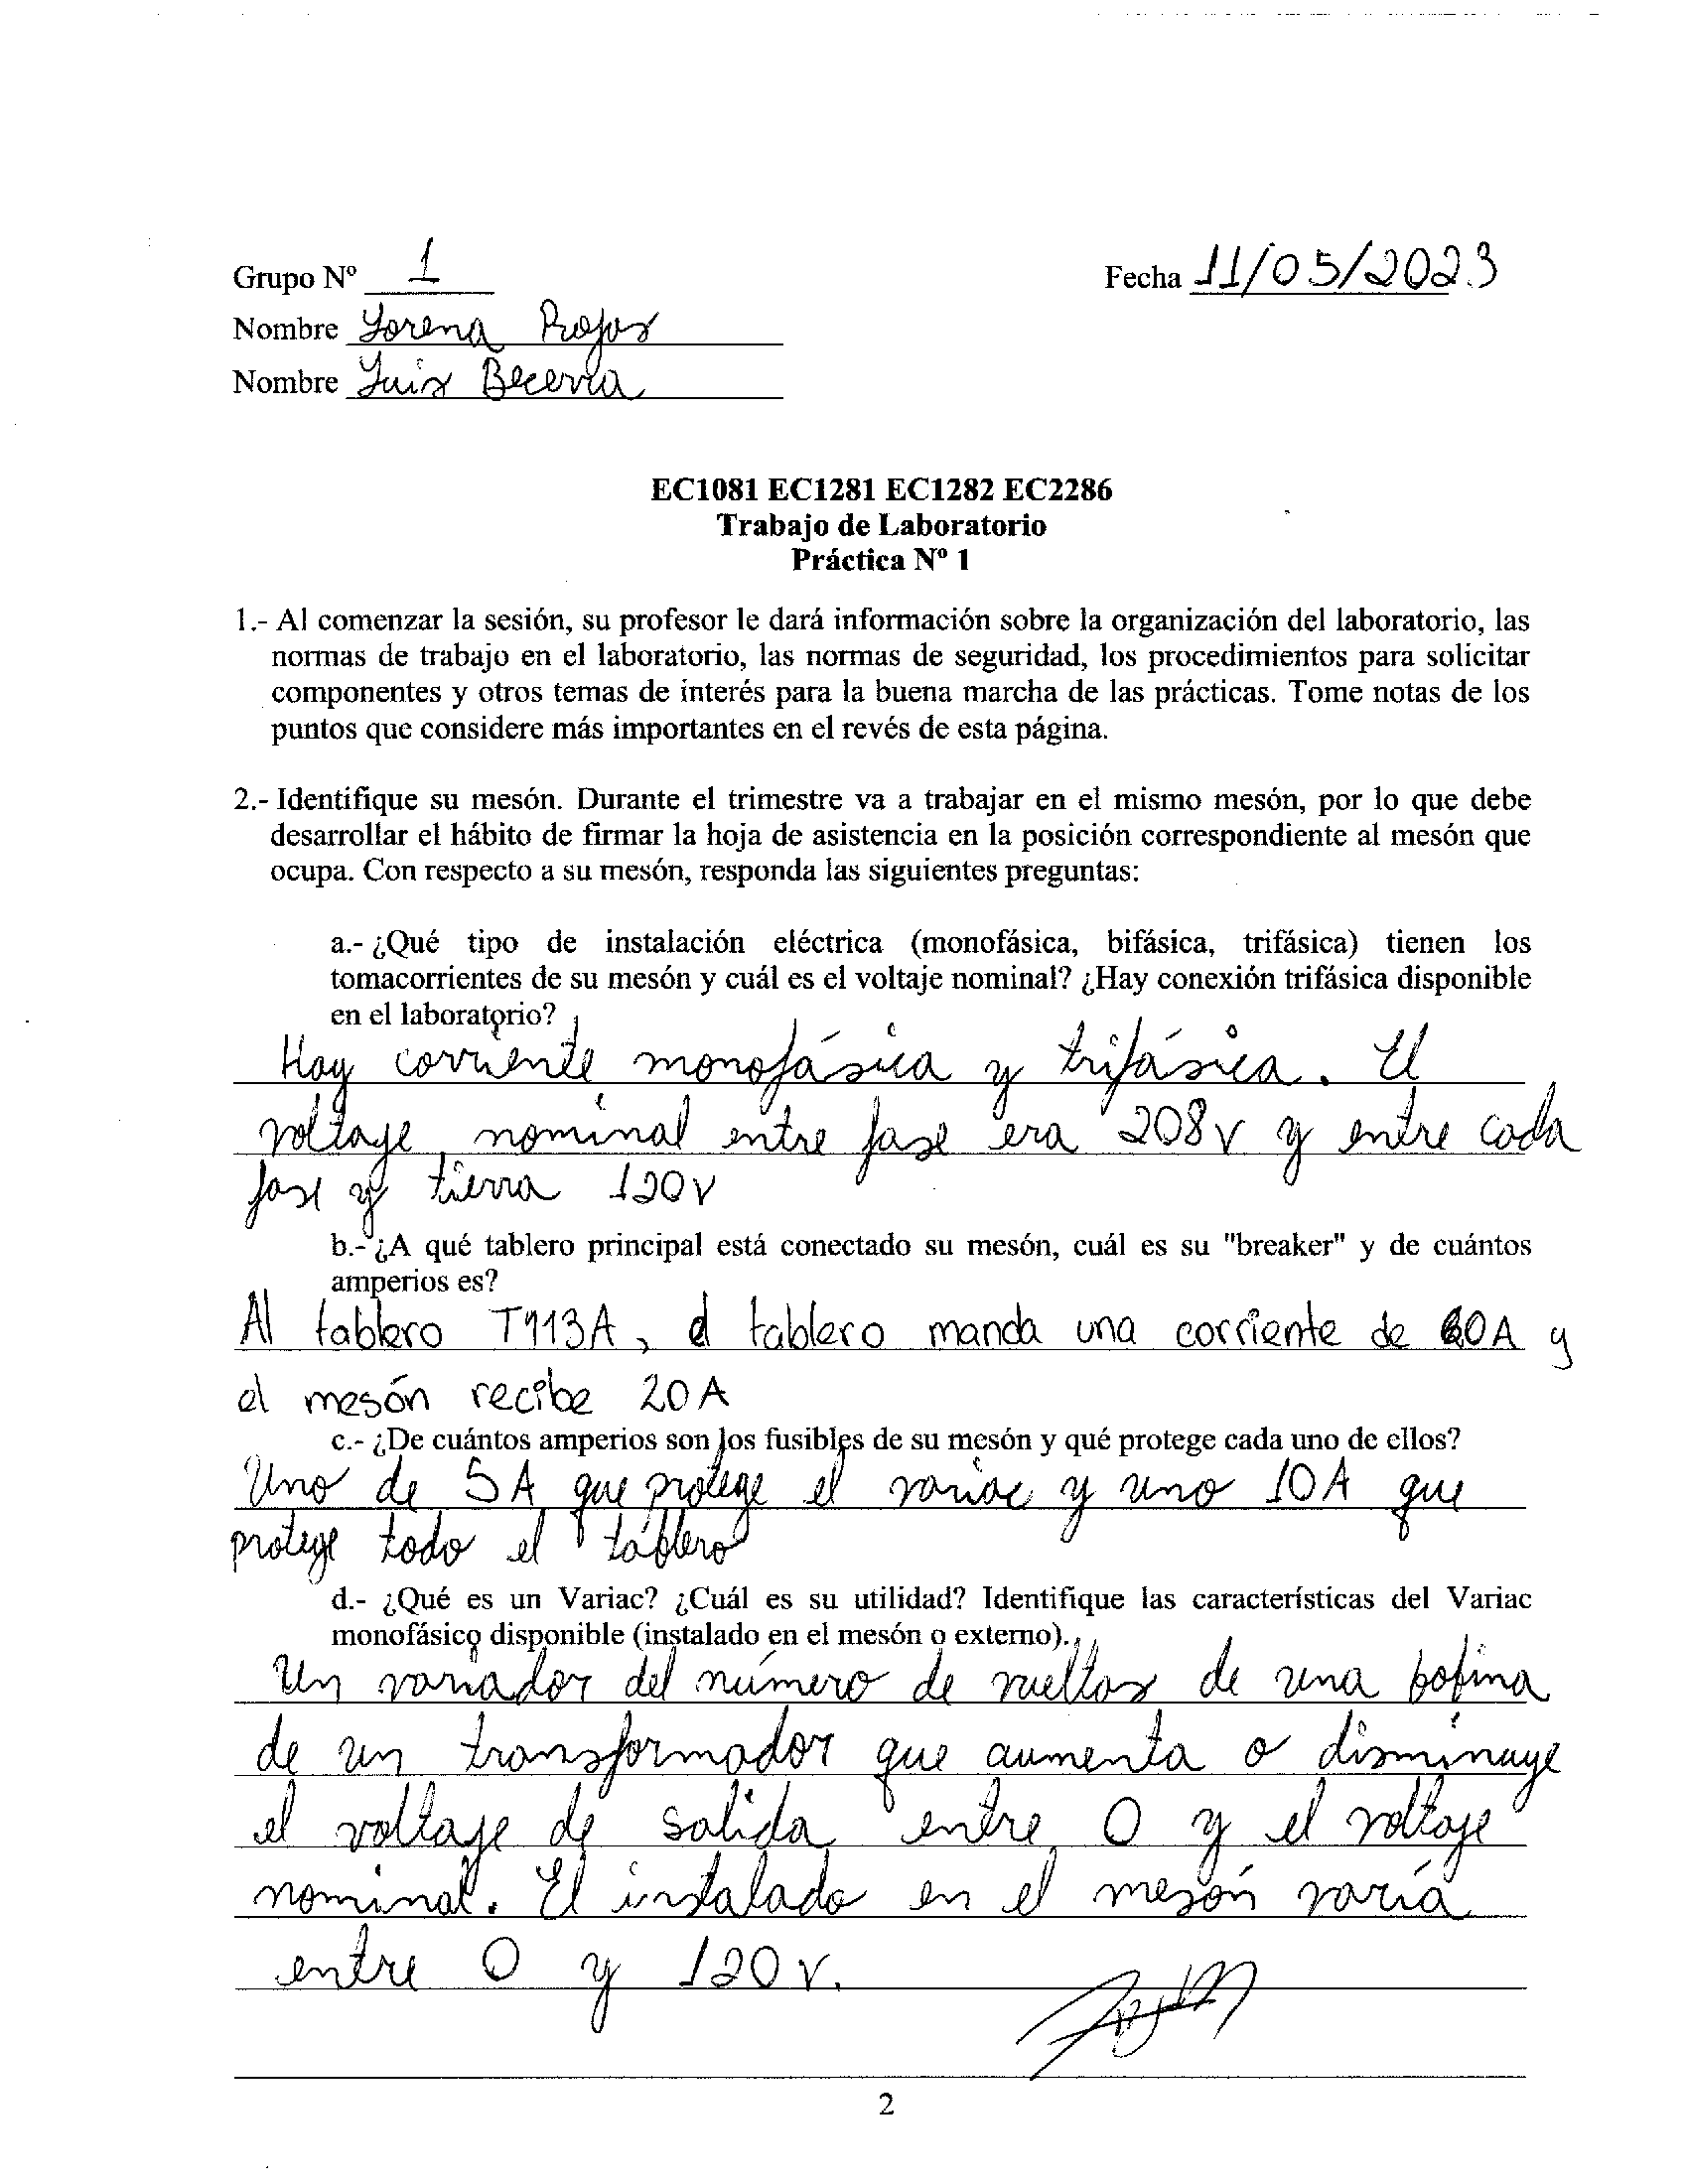
\includegraphics[width=15cm,height=20cm]{anexo1}\\
	
	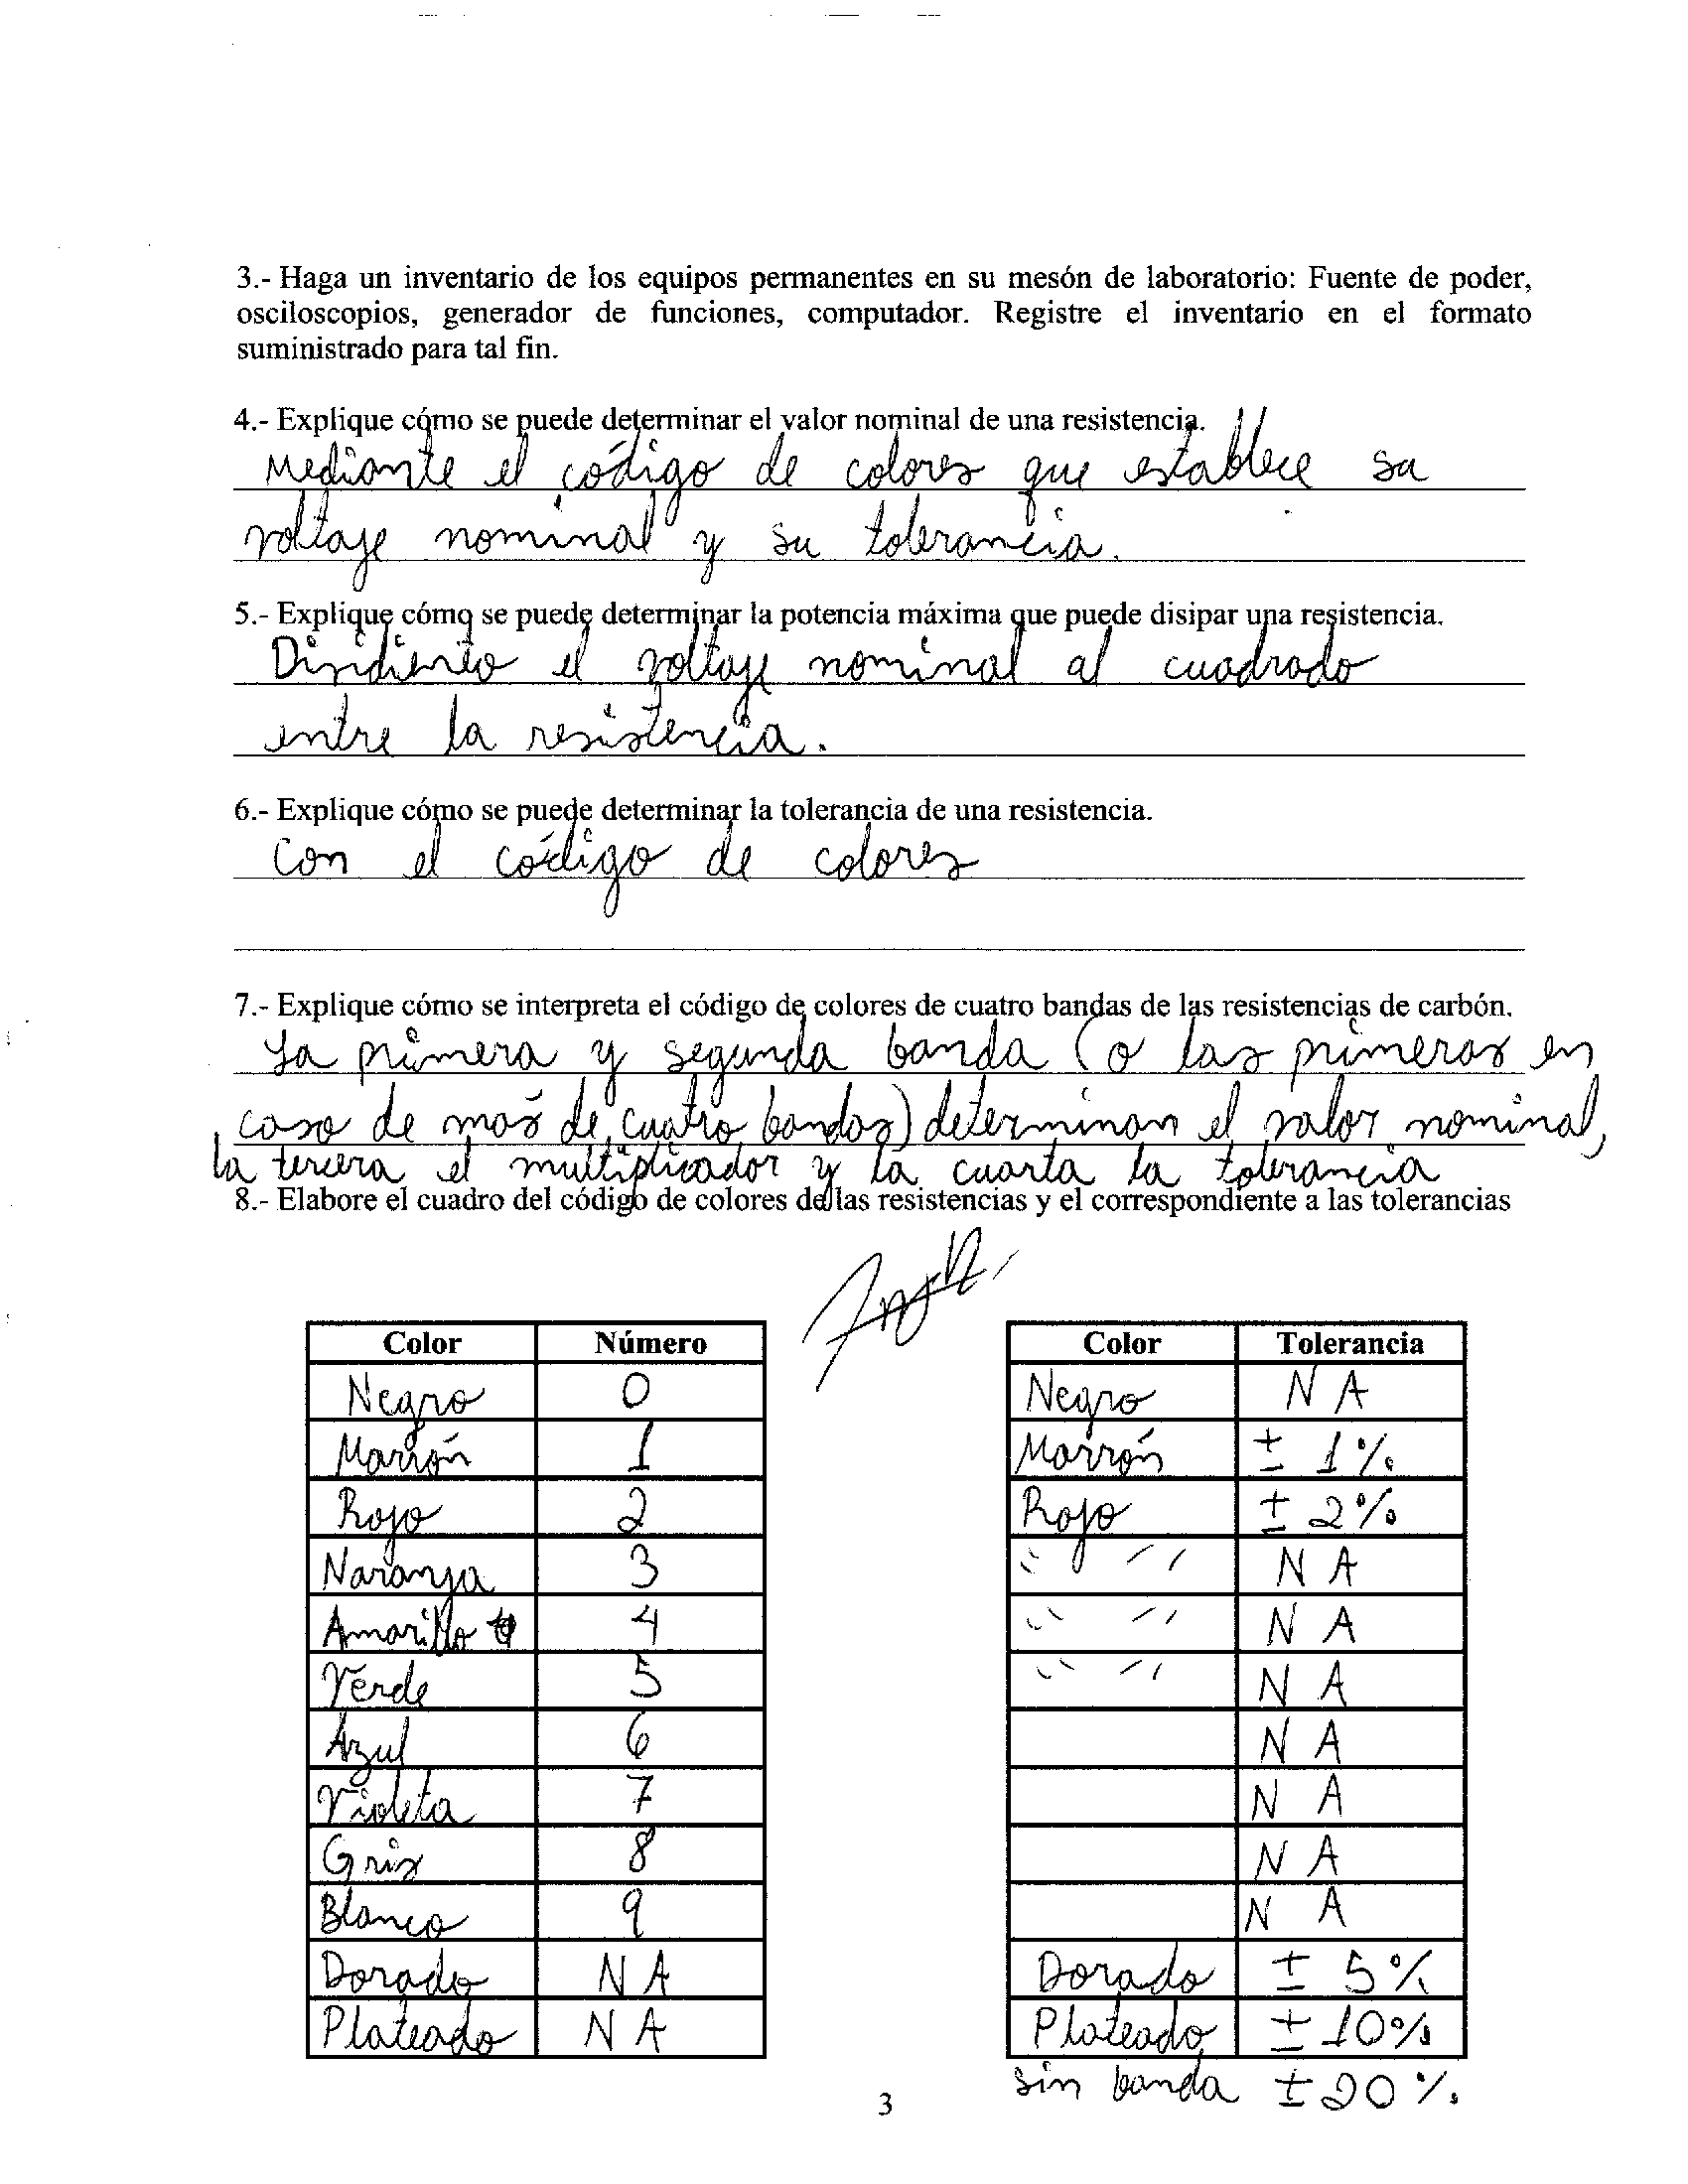
\includegraphics[width=15cm,height=20cm]{anexo2}\\
	
	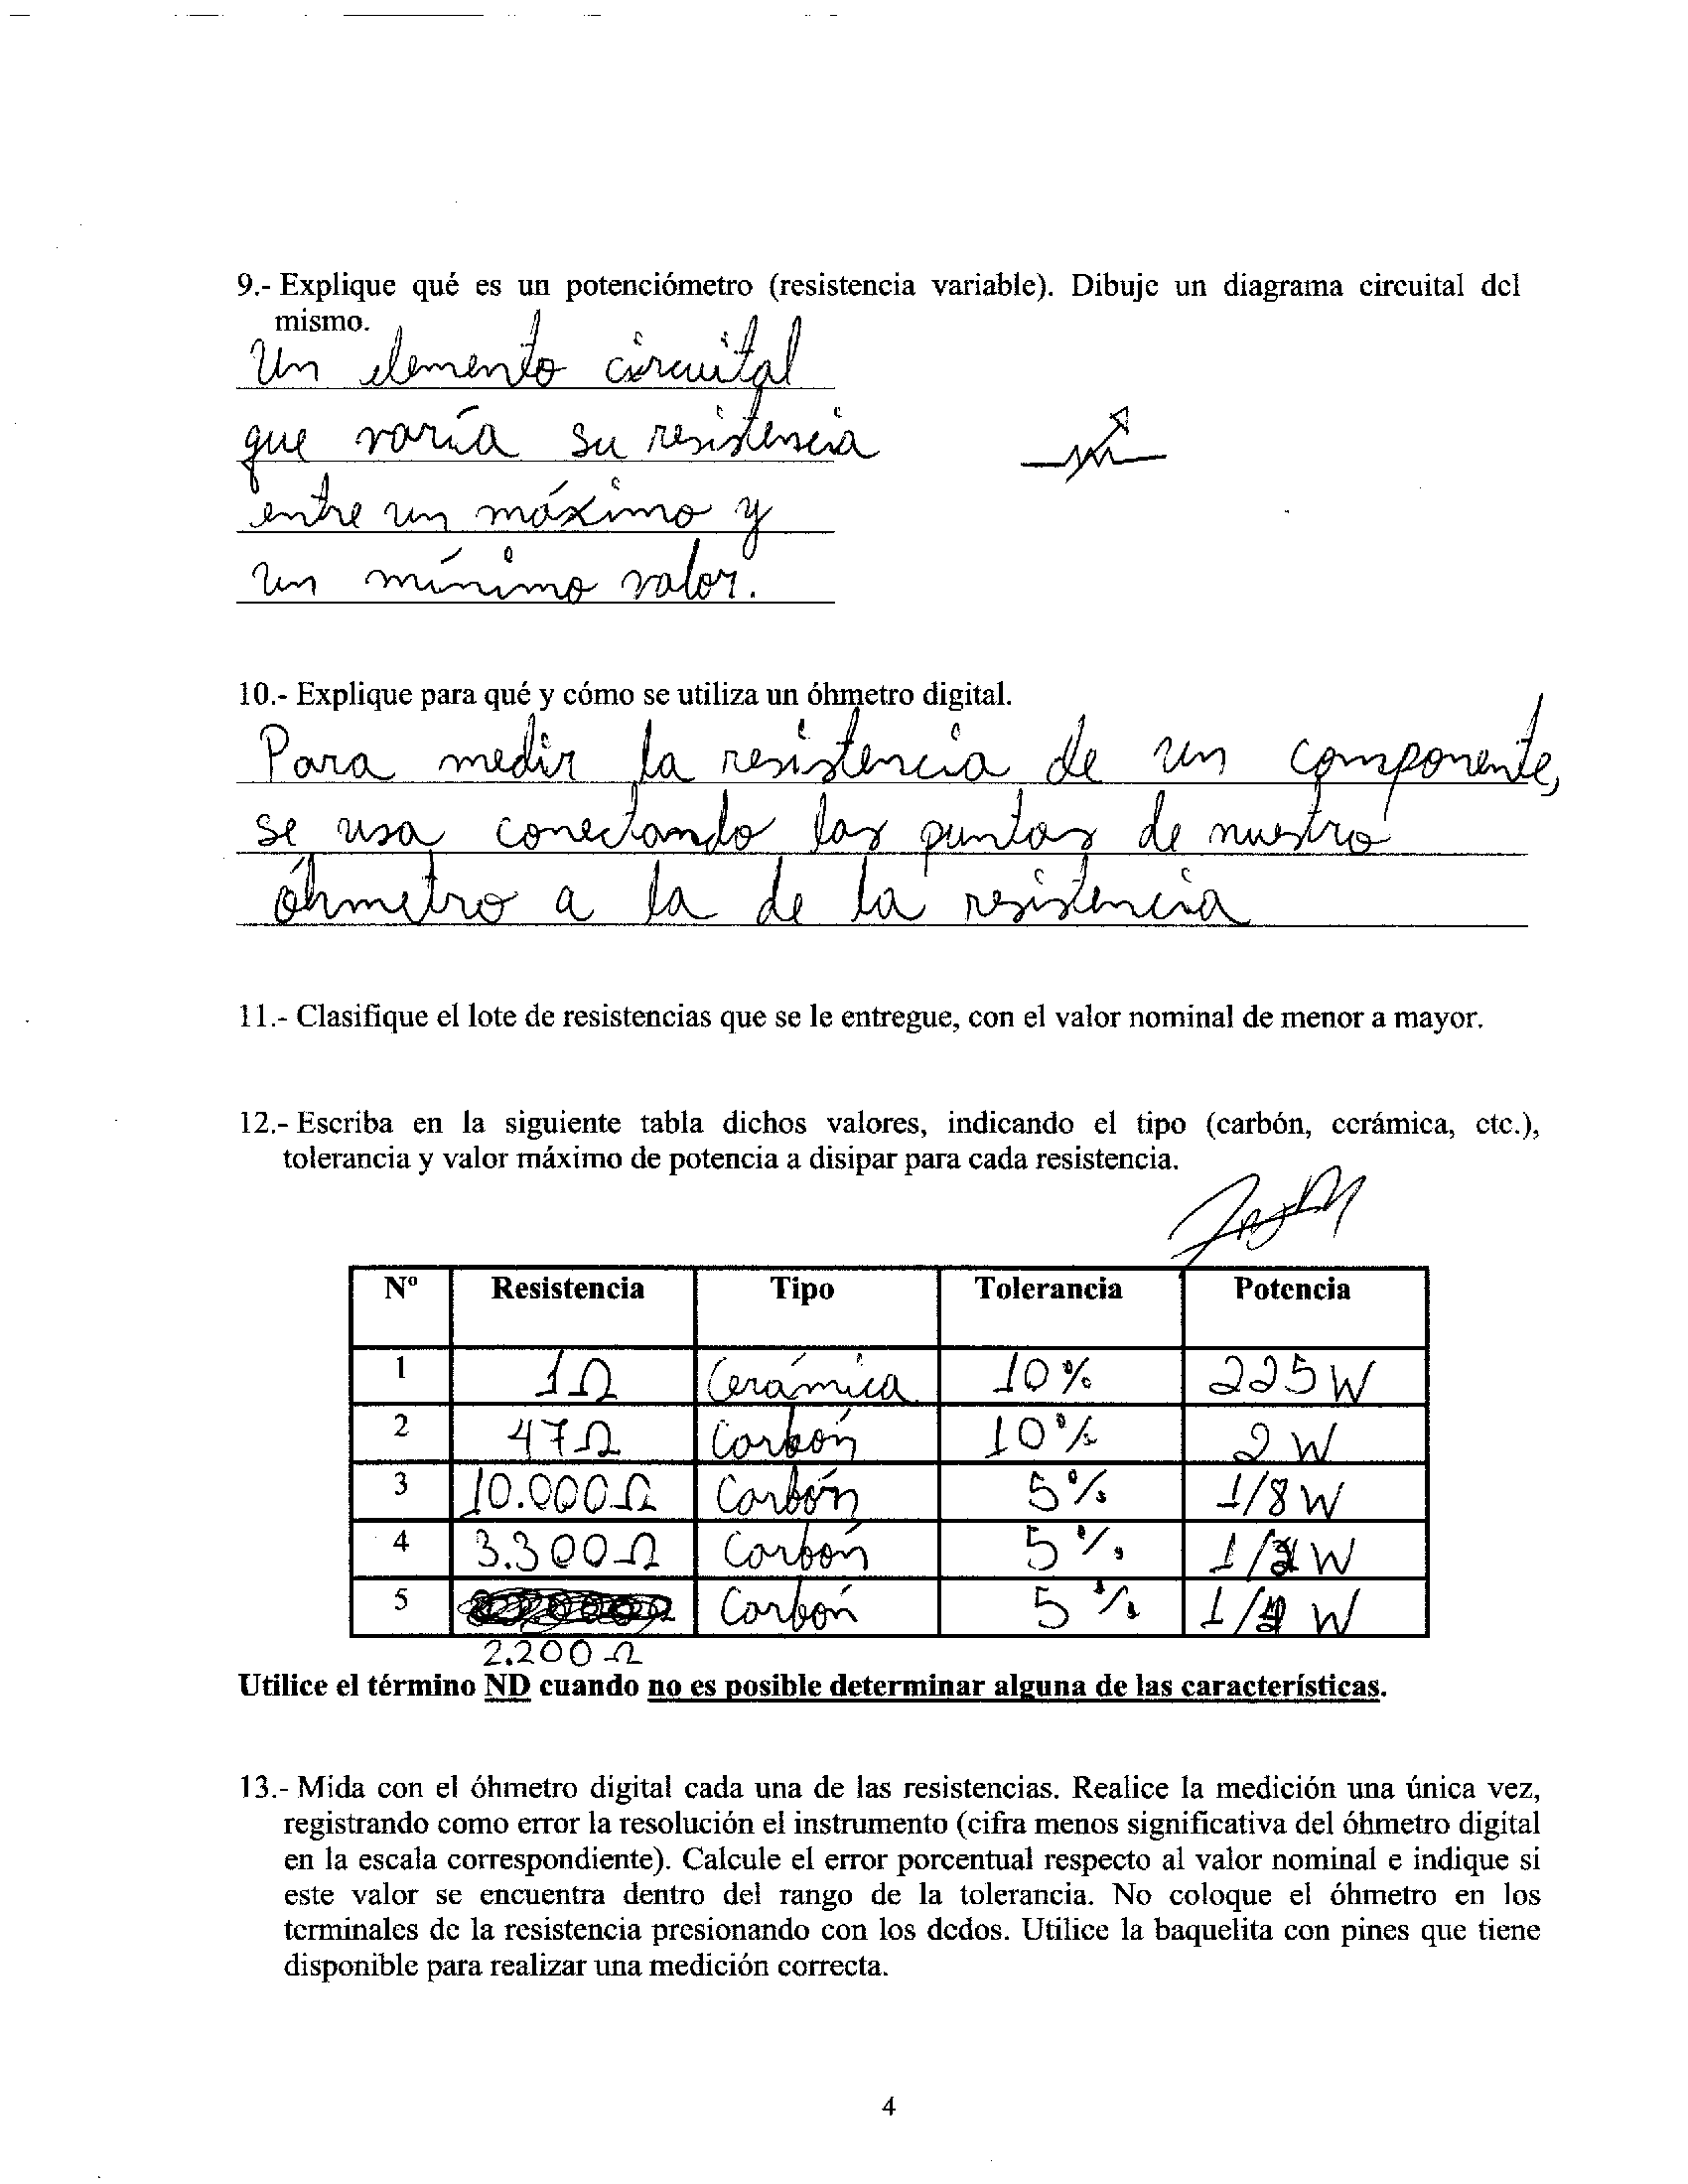
\includegraphics[width=15cm,height=20cm]{anexo3}\\
	
	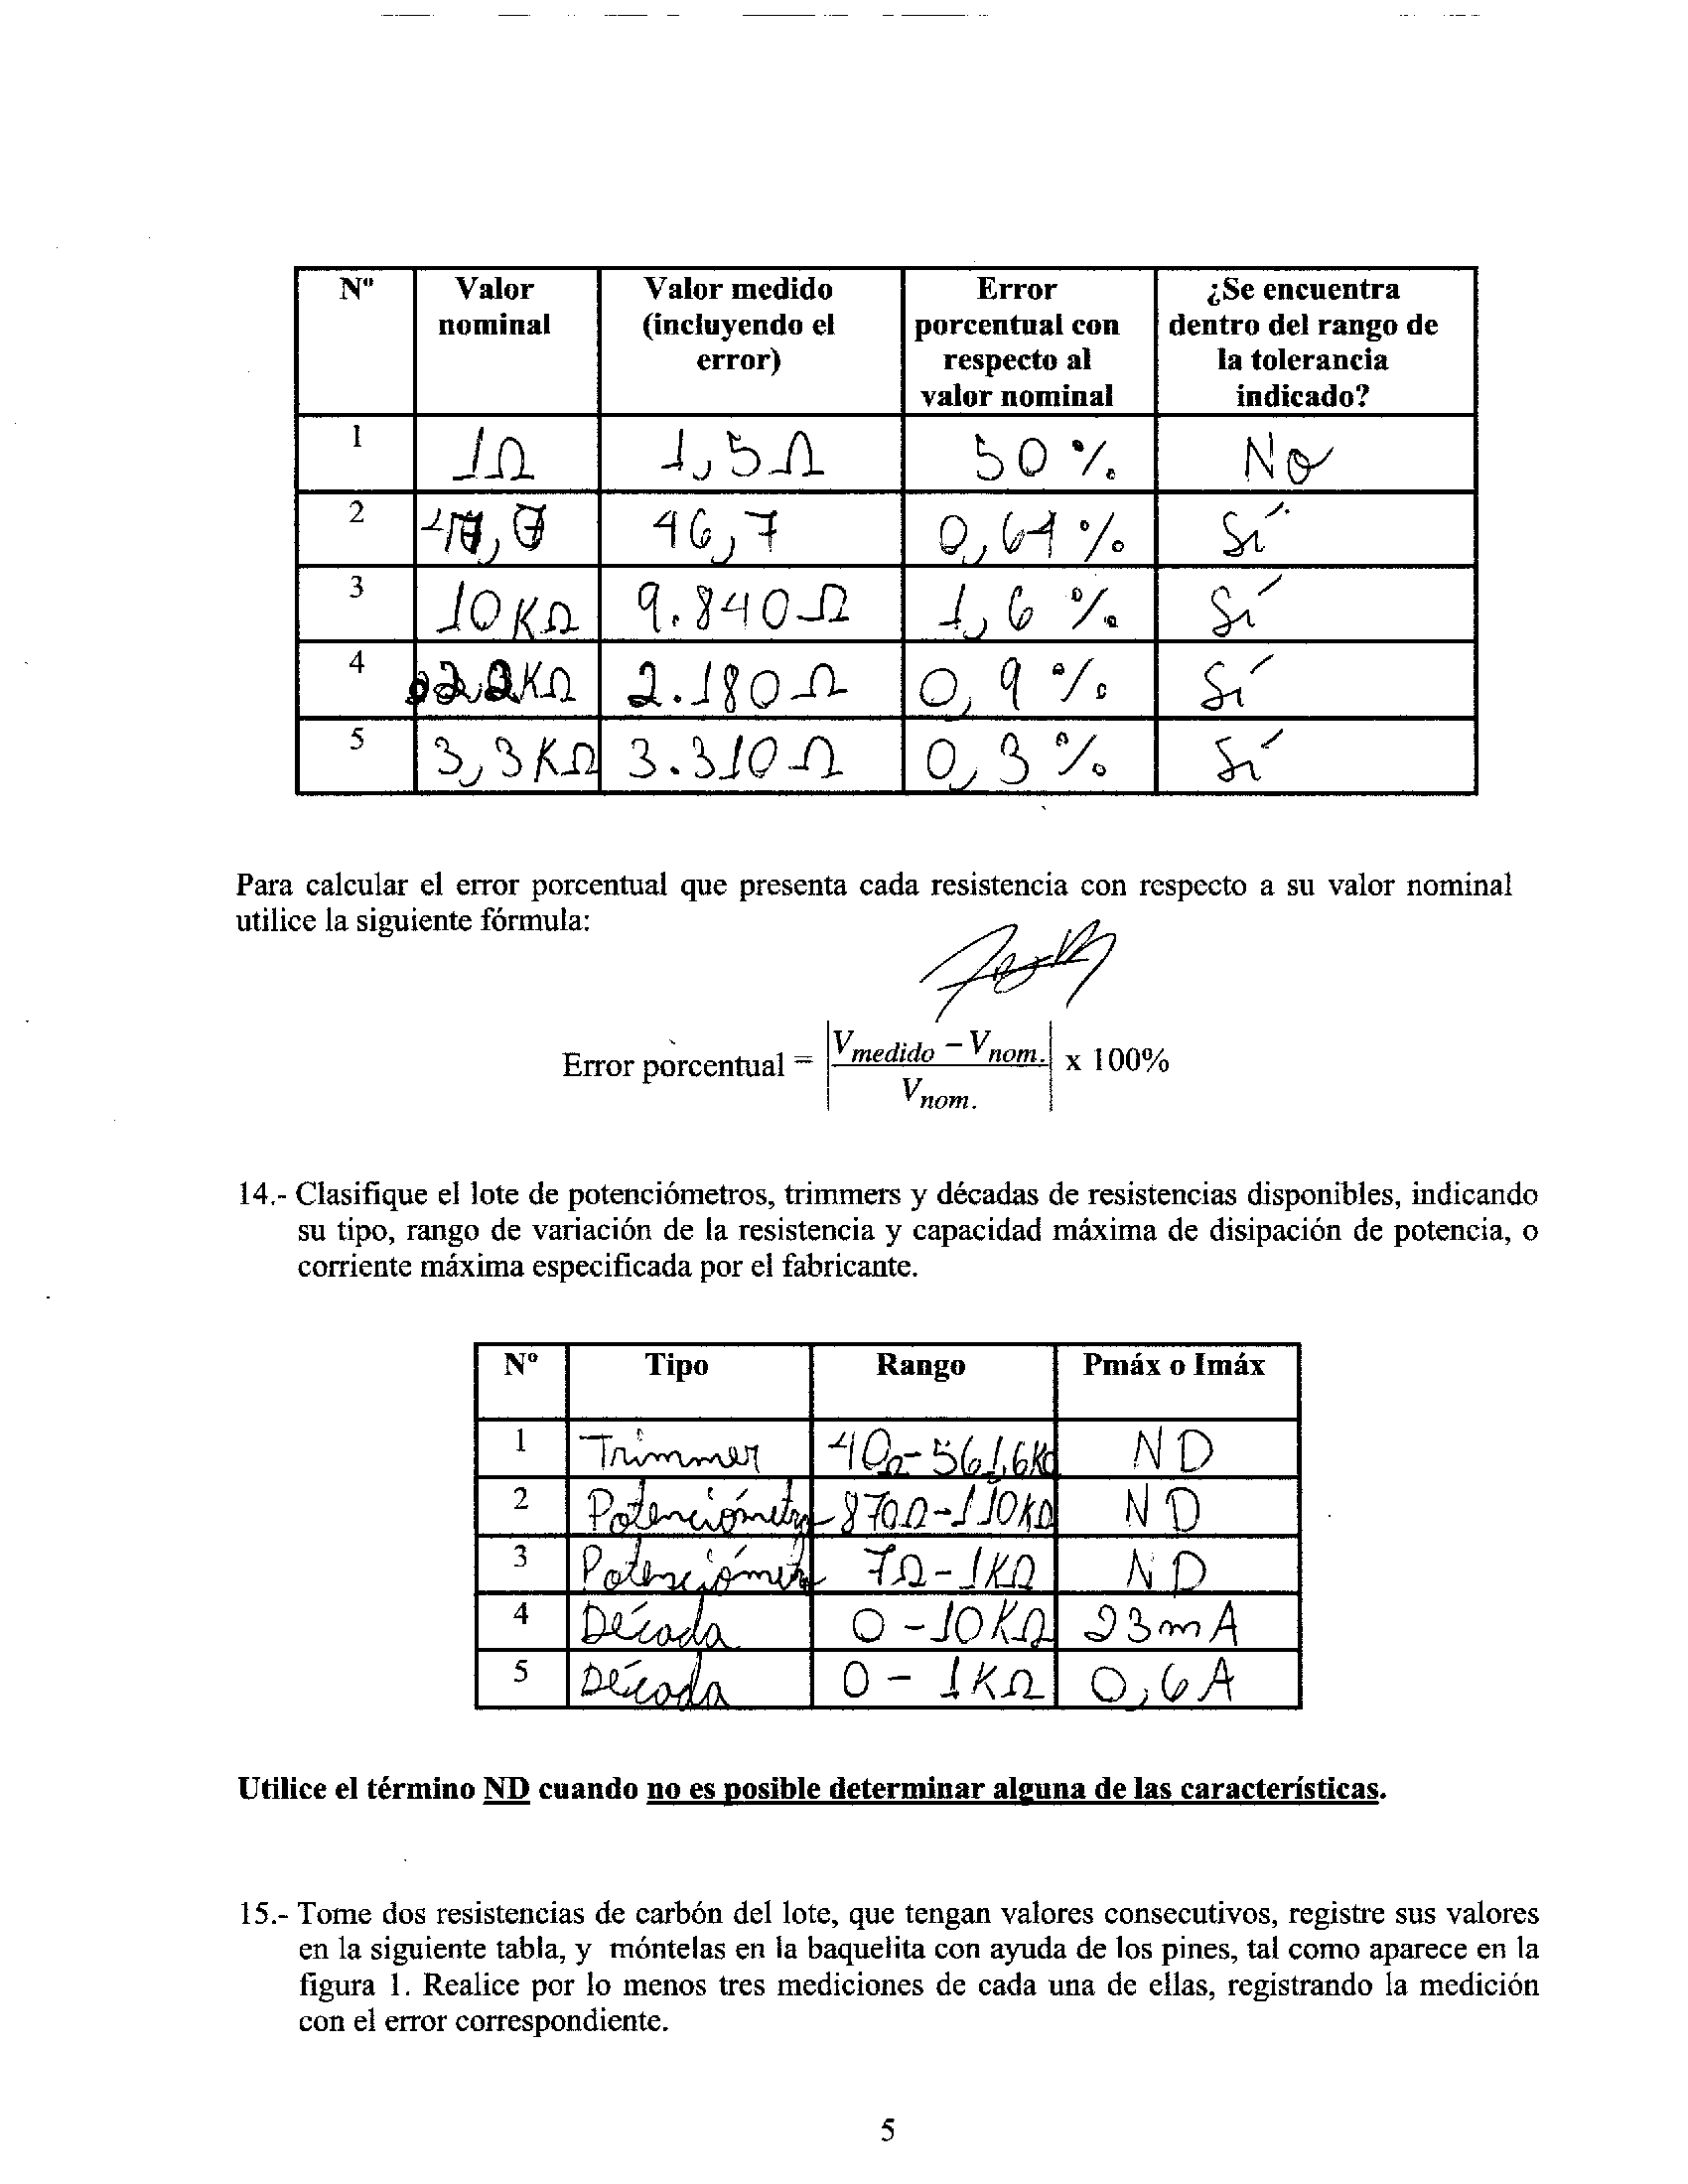
\includegraphics[width=15cm,height=20cm]{anexo4}\\
	
	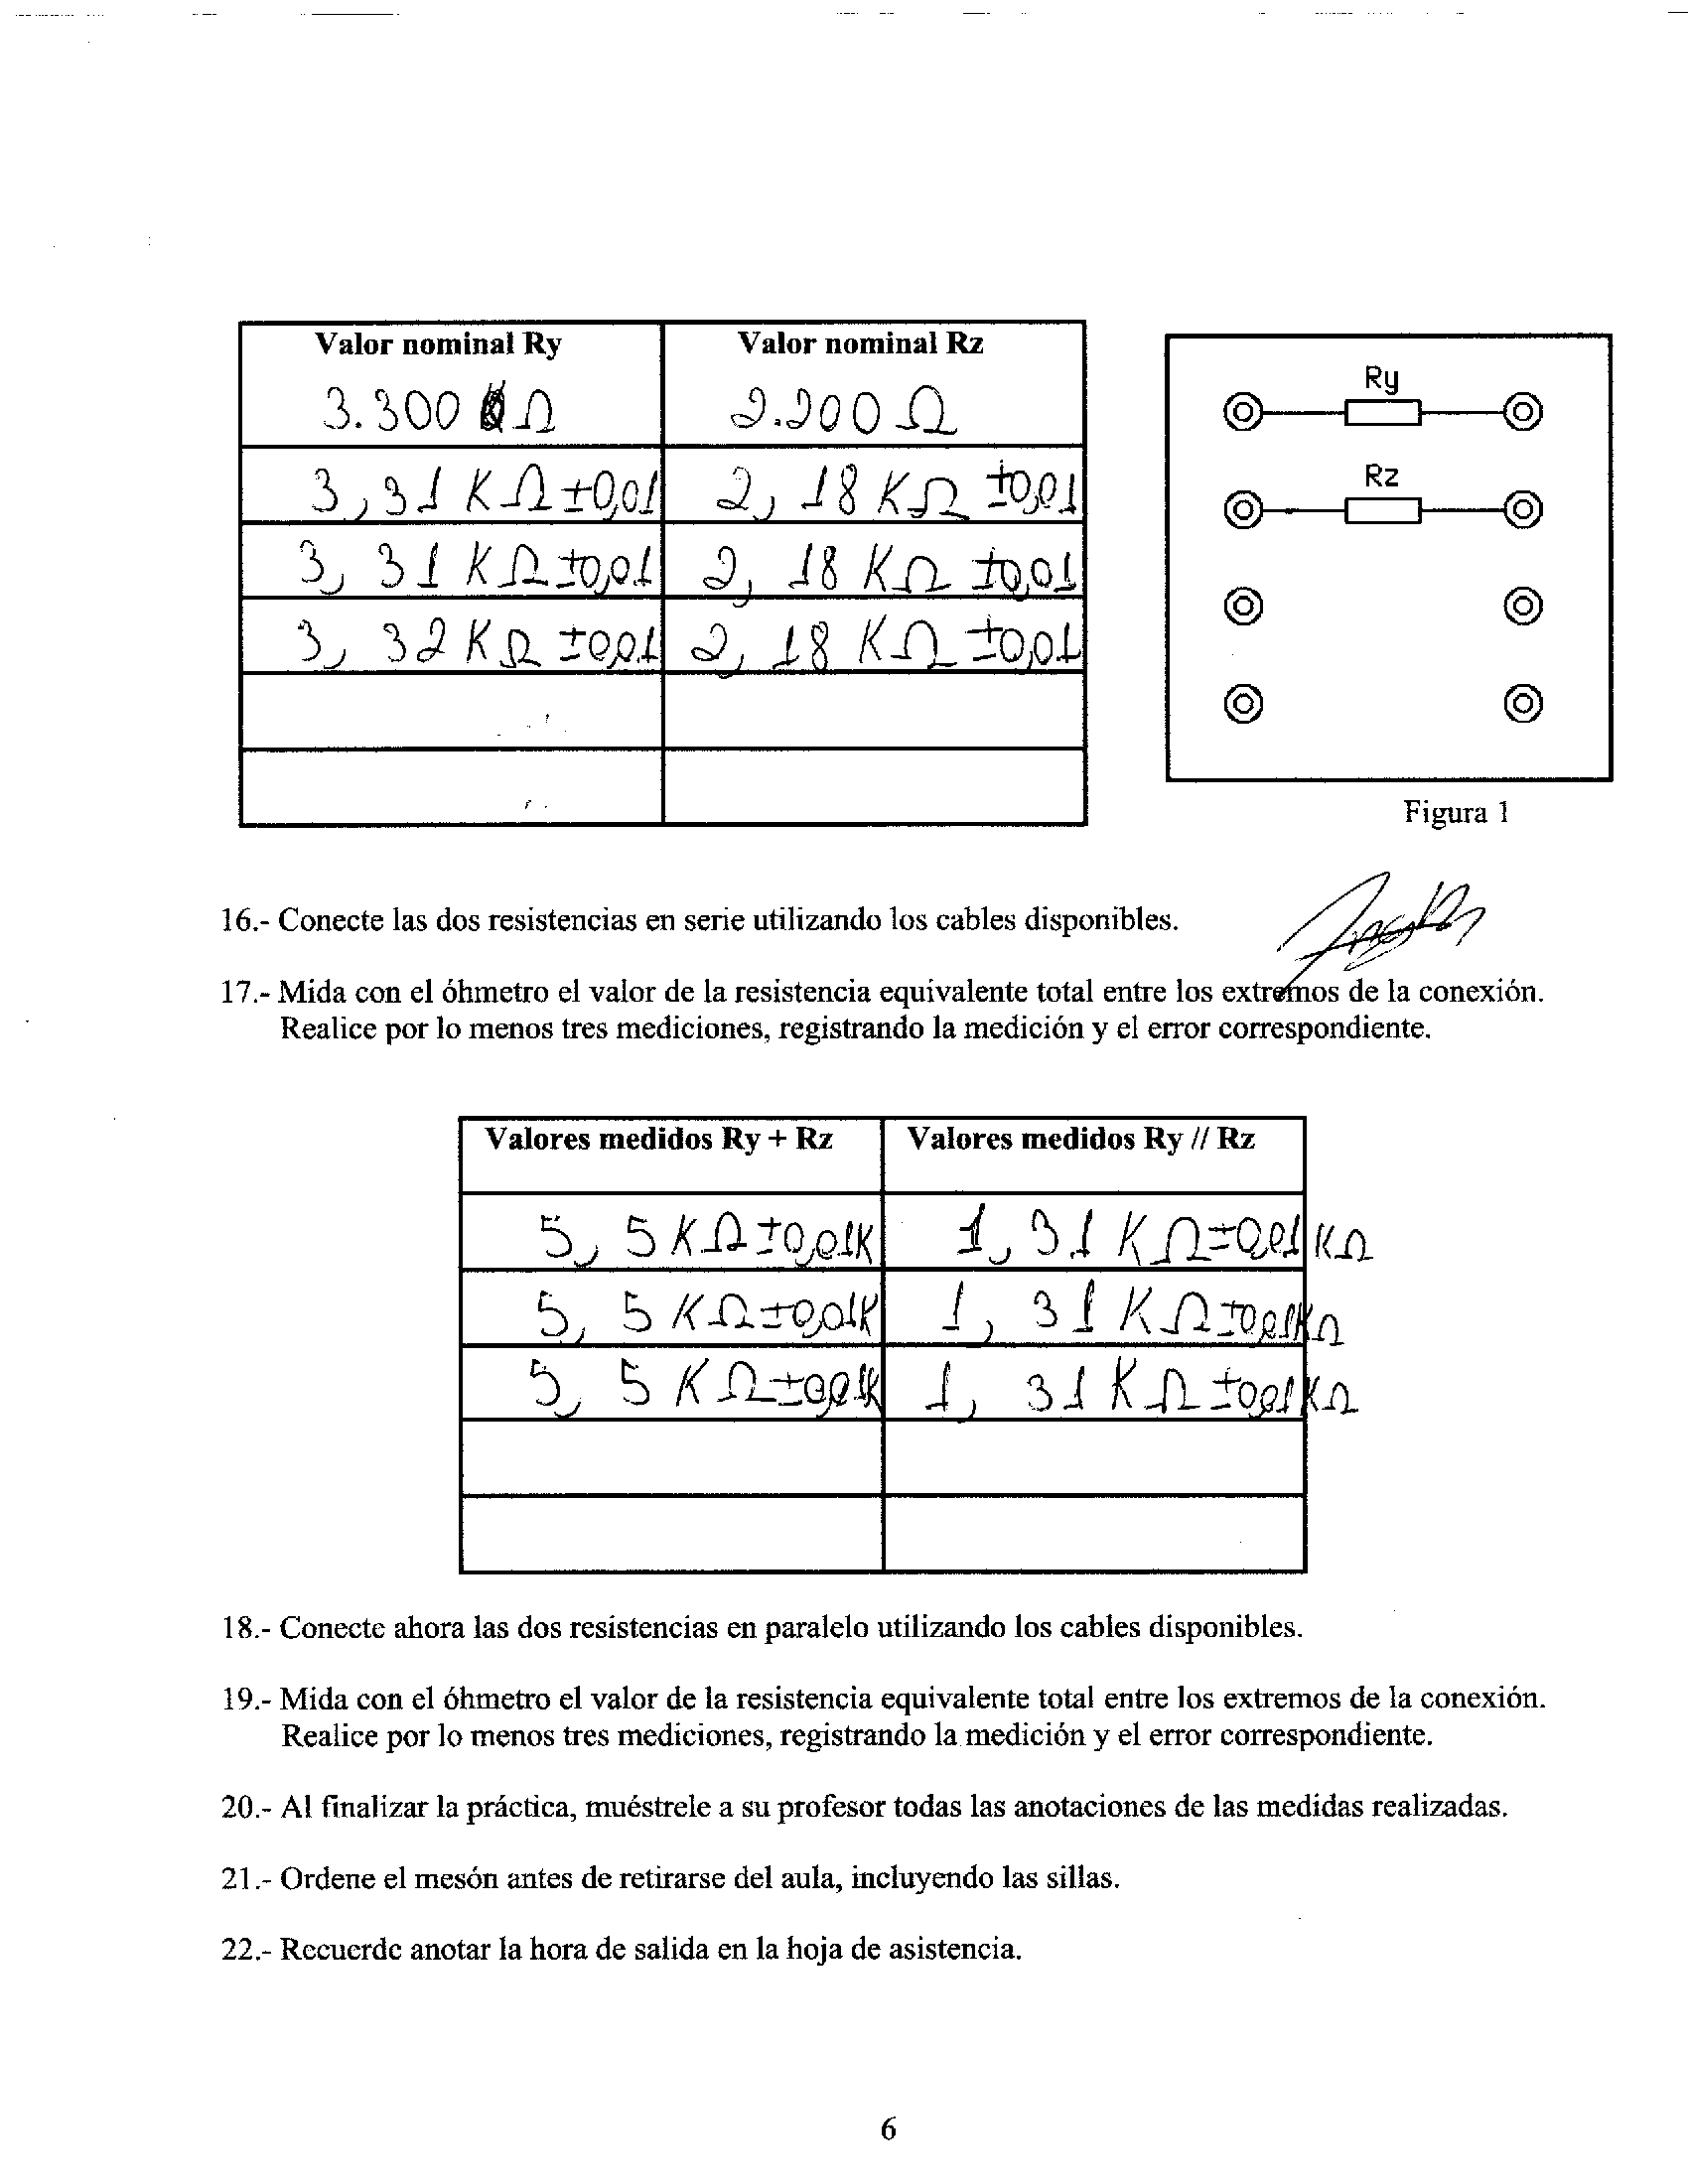
\includegraphics[width=15cm,height=20cm]{anexo5}\\
	
	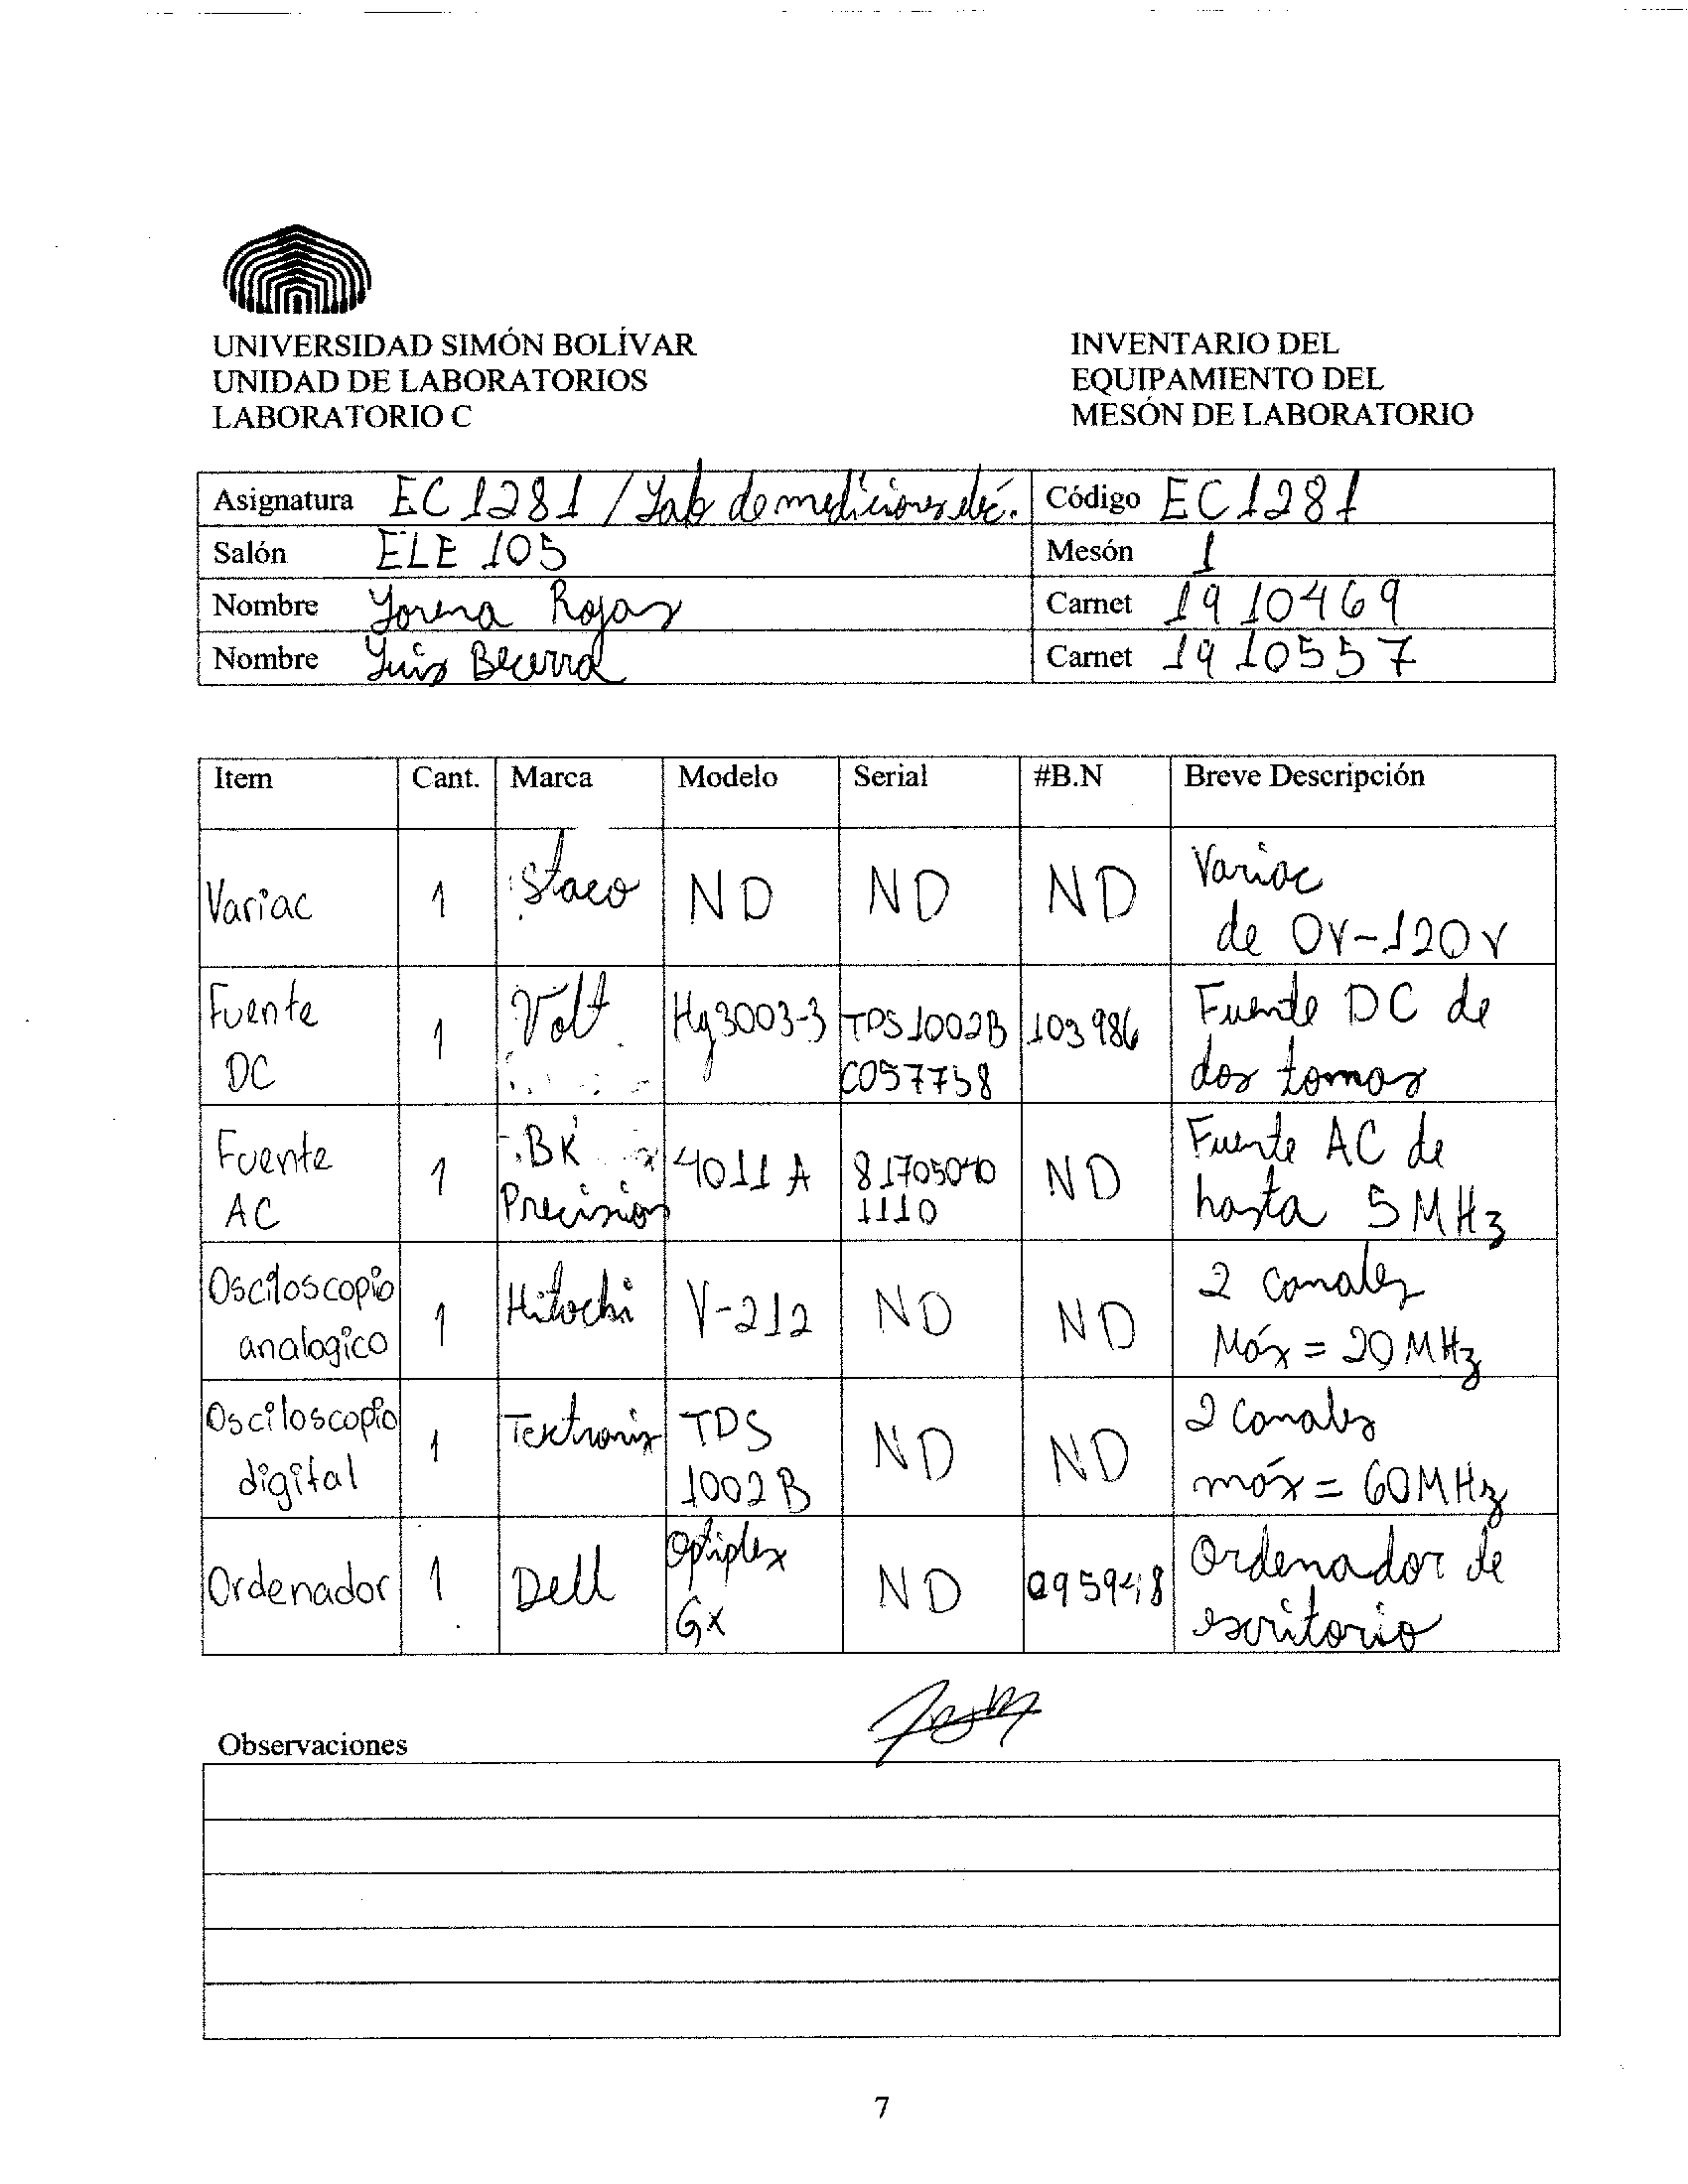
\includegraphics[width=15cm,height=20cm]{anexo6}\\
	
	\newpage
	
	\section{Cálculo de las mediciones}
	
	\subsection{Valor promedio, desviación estándar, error estándar y error total}
	
	\noindent Primero calculamos el valor promedio $<x>$ de nuestras medidas usando la fórmula $<x> = \frac{1}{n}\sum_{i=1}^n x_i$ para $R_y$ y $R_x$.
	\\
	\begin{equation}
		<R_y> = \frac{3,31 + 3,31 + 3,32}{3} k\Omega = 3,31 k\Omega
	\end{equation}
	\\
	\begin{equation}
		<R_x> = \frac{2,18 + 2,18 + 2,18}{3} k\Omega = 2,18 k\Omega
	\end{equation}
	\\
	\noindent Para el arreglo en serie usamos la fórmula $R_{eq} = \sum_{i=1}^m R_i$ donde $m$ es el número de resistencias en el arreglo y $R_i$ la resistencia i-ésima. Al aplicarlo a nuestras medidas nos queda:\\
	\begin{equation}
		<R_{xy}> = <R_y> + <R_x> = (3,31 + 2,18)k\Omega = 5,49k\Omega
	\end{equation}
	\\
	\noindent Al tratar con el arreglo de resistencias en paralelo usamos $R_{eq} = (\sum_{i=1}^m \frac{1}{R_i})^{-1}$ donde $m$ y $R_i$ son análogas a lo que se hizo anteriormente.\\
	\begin{equation}
		<R_{x||y}> = (\frac{1}{R_y} + \frac{1}{R_x})^{-1} = (\frac{1}{3,31} + \frac{1}{2,18})^{-1}k\Omega = 1,31k\Omega
	\end{equation}
	\\
	\noindent Luego calculamos la desviación estándar $S_x = \sqrt{\frac{\sum_{i=1}^n(x_i - <x>)^2}{n - 1}}$ para cada resistencia, obteniendo:\\
	\begin{equation}
		S_y = \sqrt{\frac{(3,31 - 3,31)^2 + (3,31 - 3,31)^2 + (3,32 - 3,31)^2}{3 - 1}} = 5 \times 10^{-5} k\Omega
	\end{equation}
	\\
	\begin{equation}
		S_x = \sqrt{\frac{(2,18 - 2,18)^2 + (2,18 - 2,18)^2 + (2,18 - 2,18)^2}{3 - 1}} = 0 k\Omega
	\end{equation}
	\\
	\noindent La calculamos también para las medidas de los arreglos en serie y paralelo:\\
	\begin{equation}
		S_{xy} = \sqrt{\frac{(5,5 - 5,5)^2 + (5,5 - 5,5)^2 + (5,5 - 5,5)^2}{3 - 1}} = 0 k\Omega
	\end{equation}
	\\
	\begin{equation}
		S_{x||y} = \sqrt{\frac{(1,31 - 1,31)^2 + (1,31 - 1,31)^2 + (1,31 - 1,31)^2}{3 - 1}} = 0 k\Omega
	\end{equation}
	\\
	\noindent Tendremos que para calcular el error total usaremos $\Delta Z = \sqrt{\sigma_{est}^2 + \sigma_{nom}^2}$, donde $\sigma_{est} = \frac{S_x}{\sqrt n}$ y $\sigma_{nom}$ es el error nominal determinado por el instrumento. Acá tendremos que el error nominal es equivalente al error de apreciación ya que el proceso no resultó en ningún error de definición, exactitud ni interacción.\\
	\begin{equation}
		\Delta Z_x = \sqrt{(\frac{S_x}{\sqrt n})^2 + \sigma_{nom}^2} = \sqrt{(\frac{0}{\sqrt 3})^2 + 0,01^2} = 0,01k\Omega
	\end{equation}
	\\
	\begin{equation}
		\Delta Z_y = \sqrt{(\frac{S_y}{\sqrt n})^2 + \sigma_{nom}^2} = \sqrt{(\frac{5\times 10^{-5}}{\sqrt 3})^2 + 0,01^2} = 0,01k\Omega
	\end{equation}
	\\
	\begin{equation}
		\Delta Z_{xy} = \sqrt{(\frac{S_{xy}}{\sqrt n})^2 + \sigma_{nom}^2} = \sqrt{(\frac{0}{\sqrt 3})^2 + 0,01^2} = 0,01k\Omega
	\end{equation}
	\\
	\begin{equation}
		\Delta Z_{x||y} = \sqrt{(\frac{S_{xy}}{\sqrt n})^2 + \sigma_{nom}^2} = \sqrt{(\frac{0}{\sqrt 3})^2 + 0,01^2} = 0,01k\Omega
	\end{equation}
	\\
	\subsection{Propagación de errores}
	\noindent Si bien realizamos medidas de las resistencias en serie y paralelo, es conocido que también podemos llegar a tales valores mediante operaciones con resistencias, como se hizo en páginas anteriores, a dichas medidas es necesario aplicarles la propagación de errores.
	\\
	
	\noindent Tendremos que para nuestras resistencias en serie $\Delta R_{eq} = \Delta R_x + \Delta R_y$, quedando:\\
	\begin{equation}
		\Delta R_{xy} = 0,01 + 0,01 = 0,02k\Omega
	\end{equation}
	\\
	
	\noindent Obteniendo que $R_x + R_y = 5,49k\Omega \pm 0,02k\Omega$.\\
	
	\noindent Para las resistencias en paralelo tendremos que $\Delta R_{x||y} = \frac{<R_y>^2}{(<R_x> + <R_y>)^2}\Delta R_x + \frac{<R_x>^2}{(<R_x> + <R_y>)^2}\Delta R_y$ que al desarrollar nos queda:\\
	
	\begin{equation}
		\Delta R_{x||y} = \frac{3,31^2}{(2,18 + 3,31)^2}0,01 + \frac{2,18^2}{(2,18 + 3,31)^2}0,01 = 0,005k\Omega
	\end{equation}
	\\
	
	\noindent Quedando que $R_{x||y} = 1,31k\Omega \pm 0,005k\Omega$
	
	\newpage
	
	\begin{center}
		\textbf{\large ANÁLISIS DE RESULTADOS}\\
	\end{center}
	
	\section*{Error estándar del promedio vs error nominal}
	
	\noindent A efectos de estas mediciones, se puede evidenciar que el error estandar del promedio es mínimo cuando no es cero, por lo cual la única limitante se podría decir que es la calidad de la medida de nuestra herramienta, en otras palabras, aumentar el número de medidas no representaría una mejora substancial con respecto a los resultados obtenidos con tan sólo tres medidas. \\
	
	\section*{Resultado final vs mediciones directas de los arreglos en serie y paralelo}
	
	\noindent Ambas mediciones dieron un resultado sumamente preciso, sin embargo, cabe a destacar que la medida directa fue la más precisa en el caso del circuito en serie ya que arroja la medición con un margen de error más pequeño , mientras que en el arreglo paralelo, fue la medición indirecta la que resultó en un menor error, esto se debe a que en serie,  al medir las dos resistencias, el error propagado va directamente relacionado con la suma de los dos errores medidos, mientras que en paralelo, los errores medidos se disminuyen al realizar las operaciones algebraicas.\\
	
	\section*{Rango de tolerancia de las resistencias}
	
	\noindent Las medidas tomadas revelan que los valores obtenidos sí están dentro del rango de tolerancia, luego, al proyectar eso hacia el arreglo en serie o en paralelo se encuentra con que efectivamente esta proporción se mantiene.\\
	
	\newpage
	
	\begin{center}
		\textbf{\large CONCLUSIONES}\\
	\end{center}
	
	\noindent Como se pudo observar, el manejo de los errores es un aspecto fundamental cuando se realiza un arreglo eléctrico de cualquier tipo, durante ese proceso, aunque se tengan herramientas de calidad, igualmente es indispensable ser rigurosos con las mediciones y seguir protocolos tanto por seguridad como para evitar que las medidas se vean perjudicadas por cualquier factor humano. Mientras más cautela se tenga, más se reducirá el margen de error y en consecuencia se tendrán medidas de mejor calidad.\\
	
	\noindent También cabe destacar que es excelente idea siempre que sea posible, probar con medidas directas e indirectas, ya que como se pudo evidenciar, en ocasiones una o la otra tendrá mayor precisión y si se tiene la oportunidad de probarlo, no sería una idea desacertada.\\
	
	\noindent En la medida en que se vaya avanzando, es necesario siempre tener presente que los errores son parte natural de un proceso de investigación y que si bien no se pueden erradicar, se pueden disminuir al mínimo si se siguen prácticas adecuadas al llevar a cabo cualquier tipo de experimento con arreglos eléctricos.
	
	\newpage
	
	\begin{center}
		\textbf{\large COMENTARIOS FINALES}\\
	\end{center}
	
	\noindent Esta es la primera aproximación práctica a la carrera que se tiene en ingeniería electrónica, una práctica que recuerda al rigor metodológico que se promueve durante el laboratorio de física 1 a la hora de trabajar con mediciones y presenta un abre boca de cómo se da el tratamiento de mediciones cuando se trata de fenómenos eléctricos.\\
	
	\noindent Se conocieron algunos componentes eléctricos básicos, las herramientas del laboratorio y se dió un vistazo a el procedimiento que se seguirá durante el curso para trabajar en el laboratorio, una experiencia enriquecedora y sumamente interesante.
	
\end{document}